\documentclass[11pt,a4paper]{article}
\usepackage{iftex}
\ifPDFTeX\usepackage[utf8]{inputenc}\fi
\usepackage[T1]{fontenc}
\usepackage{lmodern}
\usepackage[a4paper,margin=2.1cm,headheight=14pt]{geometry}
\usepackage{amsmath,amssymb,booktabs,graphicx,microtype,array,tabularx}
\usepackage[version=4]{mhchem}
\usepackage{xcolor}
\usepackage{tikz}
\usetikzlibrary{positioning,arrows.meta,fit,calc}
\usepackage[numbers,sort&compress]{natbib}
\usepackage{url}
\usepackage{fancyhdr}
\usepackage{enumitem}
\usepackage{caption}
\usepackage[colorlinks=true,linkcolor=blue!50!black,citecolor=blue!50!black,
  urlcolor=blue!50!black]{hyperref}
\usepackage{cleveref}

% Figures, generated tables and macros are reused from the manuscript.
\graphicspath{{../../manuscript/figures/}}
% Generated from saved completed reports.
\newcommand{\BaselineCases}{15}
\newcommand{\FollowupCases}{64}
\newcommand{\ProductionCases}{19}
\newcommand{\TimeMin}{0.0043}
\newcommand{\TimeMax}{0.323}
\newcommand{\MeshMin}{2.06}
\newcommand{\MeshMax}{10.58}
\newcommand{\ProductionResidue}{1.41\times10^{-12}}
\newcommand{\SteelLLOne}{15.35}
\newcommand{\SteelLLTwo}{8.95}
\newcommand{\SteelLLThree}{1.98}
\newcommand{\SteelUpOne}{10.47}
\newcommand{\SteelUpTwo}{10.58}
\newcommand{\SteelUpThree}{2.13}
\newcommand{\PureLLOne}{5.70}
\newcommand{\PureLLTwo}{2.15}
\newcommand{\PureUpOne}{6.57}
\newcommand{\PureUpTwo}{5.06}
\newcommand{\SteelOrderOne}{1.3}
\newcommand{\SteelOrderTwo}{3.7}
\newcommand{\SteelErrApparent}{2.5}
\newcommand{\SteelErrSecond}{3.6}
\newcommand{\SteelSmoothThree}{0.67}
\newcommand{\SteelTotalThree}{0.015}
\newcommand{\SteelCentroidRange}{0.6}
\newcommand{\SteelCentroidTRange}{0.9}
\newcommand{\UpLLOne}{20.8}
\newcommand{\UpLLTwo}{14.1}
\newcommand{\UpLLThree}{11.3}
\newcommand{\UpLLFour}{7.7}
\newcommand{\PureUpLLMin}{9.0}
\newcommand{\PureUpLLMax}{13.2}
\newcommand{\VLSteelMax}{2.8}
\newcommand{\VLPureMax}{1.8}
\newcommand{\VLSteelThree}{1.16}
\newcommand{\VLPureThree}{0.27}
\newcommand{\IterPure}{1.09\times10^{-13}}
\newcommand{\IterSteelLow}{4.89\times10^{-13}}
\newcommand{\IterSteelHigh}{0.021}
\newcommand{\LobRMS}{18}
\newcommand{\LobRMSTemp}{35}
\newcommand{\LobRMSVap}{35}
\newcommand{\LobRMSGas}{17}
\newcommand{\LobCoarse}{0.2}
\newcommand{\LobDigitised}{1.0}
\newcommand{\LobFiveInlet}{548}
\newcommand{\LobFiveGas}{+3}
\newcommand{\LobFiveGasFraction}{4.0}
\newcommand{\LobLOneMin}{0.37}
\newcommand{\LobLOneMax}{0.89}
\newcommand{\LobRMSInlet}{135}
\newcommand{\LobFiveMain}{836}
\newcommand{\LobSixDeposit}{98.1}
\newcommand{\LobFiveUpstream}{1.2}
\newcommand{\LobShiftMin}{1}
\newcommand{\LobShiftMax}{4}
\newcommand{\LobCellsProd}{22{,}896}
\newcommand{\LobCellsCoarse}{10{,}176}
\newcommand{\GraetzBound}{1.69\times10^{-12}}
\newcommand{\GraetzRuns}{45}
\newcommand{\GraetzCriteria}{27}
\newcommand{\GraetzOrderHalfMin}{1.99}
\newcommand{\GraetzOrderHalfMax}{2.00}
\newcommand{\GraetzOrderNoneMin}{1.004}
\newcommand{\GraetzOrderNoneMax}{1.008}
\newcommand{\GraetzOrderSBHalf}{2.00--2.01}
\newcommand{\GraetzOrderSBNone}{1.01--1.02}
\newcommand{\GraetzGCIHalfMax}{1.89\times10^{-4}}
\newcommand{\GraetzGCINoneMin}{0.155}
\newcommand{\GraetzGCINoneMax}{0.341}
\newcommand{\GraetzExtHalfMax}{9.47\times10^{-9}}
\newcommand{\GraetzExtNoneMax}{1.10\times10^{-5}}
\newcommand{\GraetzMuH}{7.09\times10^{-9}}
\newcommand{\LobDiffA}{+26}
\newcommand{\LobDiffB}{+19}
\newcommand{\LobDiffC}{+16}
\newcommand{\LobDiffD}{$-$11}
\newcommand{\LobDiffE}{$-$14}


\newcommand{\vect}[1]{\mathbf{#1}}
\newcommand{\units}[1]{\,\mathrm{#1}}
\newcommand{\TC}[1]{\textcolor{red}{\textbf{[TO CONFIRM: #1]}}}
\newcommand{\PENDING}[1]{\textcolor{red}{\textbf{[PENDING: #1]}}}
\newcommand{\pend}{\textcolor{red}{\textbf{[PENDING]}}}
\newcommand{\slug}[1]{\path{#1}}

\captionsetup{font=small,labelfont=bf}
\setlist{itemsep=1pt,topsep=3pt}
\setlength{\parskip}{3pt}

\pagestyle{fancy}
\fancyhf{}
\lhead{\small LESTO D38 -- Coupled GEMS and CFD codes}
\rhead{\small Version 0.1 (draft), 2026-10-14}
\cfoot{\small\thepage}

\hypersetup{pdftitle={LESTO D38: The coupled GEMS and CFD codes for fission
  products reactive transport modelling},pdfauthor={Jan Kren}}

\begin{document}

%======================================================================
\begin{titlepage}
\centering
\vspace*{1cm}
{\large LESTO -- LEad fast reactor Safety design and TOols\par}
\vspace{1.2cm}
{\Large\bfseries Deliverable D38\par}
\vspace{0.6cm}
{\LARGE\bfseries The coupled GEMS and CFD codes for fission products
reactive transport modelling\par}
\vspace{0.4cm}
{\large Description of the developed coupling and modelling\par}
\vspace{1.2cm}
{\large Jan Kren\par}
{Paul Scherrer Institute (PSI), 5232 Villigen PSI, Switzerland\par}
\vspace{1.2cm}

\renewcommand{\arraystretch}{1.25}
\begin{tabularx}{0.9\textwidth}{>{\bfseries}l X}
\toprule
Project & LESTO (LEad fast reactor Safety design and TOols)\\
Grant agreement no. & \TC{EU grant agreement number}\\
Deliverable & D38 \\
Title & The coupled GEMS and CFD codes for fission products reactive
        transport modelling\\
Work package / task & \TC{work package number and title}; Task 3.4\\
WP leader / task leader & \TC{WP leader}; \TC{Task 3.4 leader}\\
Lead beneficiary & \TC{lead beneficiary of D38}\\
Contributing partner & Paul Scherrer Institute (PSI)\\
Author & Jan Kren (PSI)\\
Contractual due date & Month 24, \TC{calendar due date}\\
Nature & \TC{deliverable type (e.g.\ report, software)}\\
Dissemination level & \TC{dissemination level}\\
Version, date & 0.1 (draft), 2026-10-14\\
Reviewed by & \TC{internal reviewers}\\
\bottomrule
\end{tabularx}

\vspace{0.8cm}
\begin{tabularx}{0.9\textwidth}{l l X}
\toprule
\textbf{Version} & \textbf{Date} & \textbf{Change}\\
\midrule
0.1 & 2026-10-14 & First draft for internal review.\\
\bottomrule
\end{tabularx}

\vfill
{\small\TC{funding acknowledgement and EU disclaimer text required by
the grant agreement}\par}
\end{titlepage}

%======================================================================
\section*{Executive summary}
\addcontentsline{toc}{section}{Executive summary}

This deliverable describes the coupling of the OpenFOAM finite-volume
solver \texttt{rhoFixedFlowFoam} with the GEMS3K Gibbs-energy
minimisation kernel \cite{Kulik2013gemselektor}, developed at PSI for
the reactive transport of volatile fission-product species. The test
bed is the thermal-gradient (thermosublimatography) column, in which
iodine compounds evaporated from lead--bismuth eutectic (LBE) are carried
by helium along a falling wall temperature and deposit by volatility
\cite{Liu2025chemical,Lobresco2026assessment}.

\textbf{What was developed.} (i) A transport solver for any number of
trace gases in a frozen helium carrier, with reversible
Hertz--Knudsen--Schrage (HKS) wall exchange in series with the near-wall
diffusion resistance, shared condensed wall inventories, a reactive
BiI wall channel and an exact element ledger for Pb, Bi and I. (ii) A
plain-C bridge to GEMS3K that links a static GEMS3K into the OpenFOAM
executable. (iii) Two coupling points: GEMS3K equilibrium pressures for
the HKS law, and homogeneous gas re-speciation of nine Pb--Bi--I gases
per cell by three engines: an exact ideal-gas element-potential kernel,
GEMS3K standard states with that kernel (\emph{frozen}), and warm
per-cell GEMS3K calls refined by the kernel (\emph{local}). (iv)
GEMS3K input systems for Pb--I--He and Pb--Bi--I--He generated from
thermodynamic records without GEM-Selektor.

\textbf{What was established.} The coupled code conserves elements to
round-off: the largest raw element residue of the 19 production runs is
$\ProductionResidue$ of the supplied material. On a qualification channel
the frozen engine reproduces the kernel deposits within
$1.1\times10^{-7}$ (L1) and the local engine reproduces the frozen one
exactly; 5,814,420 local calls cost $132\units{\mu s}$ each on average.
Mapping GEMS3K over 321,480 Pb--Bi--I and Pb--I calls showed that its interior-point
method stalls in hot, non-dilute Bi-iodide gas and is silently
inaccurate for trace species; the coupling therefore guards every call and
refines or replaces it by the exact kernel. The production results
reported here use the exact kernel with formation constants generated
from the same standard-state data as the GEMS3K system; a full-size
per-cell GEMS3K run of the full production case (41,472 cells, 60\,s)
reproduces the kernel deposits within $2.1\times10^{-4}$ (L1), the order
of parallel round-off; its 514.5 million GEMS3K calls all succeeded, and
the final speciation is computed by the kernel from GEMS3K's
thermodynamic data (\cref{sec:pending}).

\textbf{Modelling results.} Applied to Liu et al.\ (2025)
\cite{Liu2025chemical}, the model places all five computed binned iodide
peak temperatures inside the printed experimental ranges; the comparison
is conditional, because the source masses are taken from the same
deposits. The computed BiI$_3$/PbI$_2$ split depends strongly on BiI(g)
thermodynamics: a $+29\units{kJ\,mol^{-1}}$ surrogate shift changes the
BiI$_3$ share of deposited iodide iodine from 94.58\% to 2.01\%. Without
tuning, the same wall law reproduces the deposition-onset temperatures
of five PbI$_2$ experiments of Lobresco et al.\ (2026)
\cite{Lobresco2026assessment} with an RMS deviation of \LobRMS{} K,
against \LobRMSTemp{} K for both models of that study. These are
verification and conditional comparisons, not a validation of the
model.

\setcounter{tocdepth}{1}
\tableofcontents

%======================================================================
\section{Introduction}
\label{sec:intro}

\paragraph{Purpose within Task 3.4.} Task 3.4 of LESTO addresses the
release and transport of fission products from the coolant source. The
approach of PSI combines computational fluid dynamics (CFD) with
chemical-thermodynamic equilibrium computed by GEMS/GEMS3K
\cite{Kulik2013gemselektor,Wagner2012gemselektor}, following earlier
CFD--GEM coupling for reactor coolant chemistry
\cite{Marino2020multiphysics}. This deliverable documents the coupled
code as built: its equations and data flow, the coupling interface, its
verification, and its first modelling applications.

\paragraph{The physical problem.} Iodine released from LBE can travel as
several gaseous species (Pb, PbI, PbI$_2$, Bi, Bi$_2$, BiI, BiI$_3$,
I, I$_2$) before it deposits on cooler surfaces. The chemical form sets
both the gas inventory available for transport and the equilibrium
pressure that governs wall exchange. Thermal-gradient columns separate
volatile species along a falling wall temperature and provide spatially
resolved deposition data \cite{Liu2025chemical,Lobresco2026assessment,
Eichler1975verfluchtigung,Zvara2008inorganic}. In fluid-dynamic terms,
a column is a slow laminar helium flow ($\mathrm{Re}\approx0.7$--3) in a
narrow tube, where axial advection, radial diffusion to the wall and a
nonlinear, temperature-dependent wall exchange together set the deposit
profile (\cref{fig:geometry}).

\paragraph{What D38 delivers.}
\begin{itemize}
\item The CFD solver \texttt{rhoFixedFlowFoam} for OpenFOAM v2412 and
  v2606, with
  multi-species transport, wall exchange and element accounting
  (\cref{sec:cfd}).
\item The GEMS3K coupling: bridge library, input-system generator,
  coupling points, guards and fallbacks, with measured robustness and
  cost (\cref{sec:coupling}).
\item A regression and verification suite and the numerical studies
  of the production cases (\cref{sec:verification}).
\item Two modelling applications, Liu et al.\ (2025) and Lobresco et
  al.\ (2026) (\cref{sec:applications}), and a reproducible case ladder
  (\cref{sec:availability}).
\end{itemize}
A methods manuscript based on the same results is in preparation; this
report reuses its figures and generated tables.



%======================================================================
\section{The CFD code: rhoFixedFlowFoam}
\label{sec:cfd}

\paragraph{Frozen carrier.} The carrier fields $\rho$, $\vect u$, $T$,
$p$ and the face mass flux $\phi$ are taken from a converged steady
laminar helium calculation with \texttt{rhoSimpleFoam} and are held
fixed. A flux-potential projection removes residual discrete divergence
before species transport, and continuity is checked to $10^{-12}$ of the
inlet flow. No momentum, pressure or energy equation is solved during
species transport, so the trace species do not feed back on the carrier.

\paragraph{Species transport.} Each gas $i$ is carried as a mass ratio
$Y_i$ and satisfies
\begin{equation}
 \frac{\partial(\rho Y_i)}{\partial t}+\nabla\cdot(\rho\vect u Y_i)
 =\nabla\cdot(\rho D_i\nabla Y_i)+S_i^{\rm rel}+S_i^{\rm wall},
 \label{eq:transport}
\end{equation}
with implicit Euler time integration, a run-time selectable advection
scheme and constant, PbI$_2$--He or Chapman--Enskog diffusivities.
Species are defined at run time; adding a species needs no recompilation.
Each species carries a chemical formula, checked against its molar mass,
from which the element concentrations
$b_k=\sum_i\nu_{ki}\rho Y_i/M_i$ ($k\in\{\mathrm{Pb,Bi,I}\}$) are
formed.

\paragraph{Wall exchange.} A gas is paired with a condensed species
stored as an immobile inventory on each wall face (an \emph{element}).
The exchange law is affine in the cell value, $q_e=a_e-g_eY_c$, and is
assembled implicitly. Two laws are implemented:
\begin{itemize}
\item the \emph{temperature model}, a temperature-activated deposition
  velocity $v_d[1-e^{-k(T_{\rm dep}-T_e)}]^+$, as in the
  temperature-based model of Lobresco et al.\
  \cite{Lobresco2026assessment};
\item the \emph{HKS law} \cite{Hertz1882verdunstung,Knudsen1915maximale,
  Schrage1953theoretical}, $j_i=G_i[p_{{\rm eq},i}(T_w)-p_{i,w}]$ with
  $G_i=C_es_i\,\tfrac{2\alpha_i}{2-\alpha_i}\sqrt{M_i/(2\pi RT_w)}$,
  placed in series with the diffusion over the cell-centre-to-wall
  distance $d_f$:
  \begin{equation}
   G_{i,f}^{\rm eff}=\frac{G_i}{1+G_i\chi_{i,c}d_f/(\rho D_i)_f},
   \qquad j_{i,f}=G_{i,f}^{\rm eff}
   \bigl[p_{{\rm eq},i}(T_w)-\chi_{i,c}Y_{i,c}\bigr],
   \label{eq:halfcell}
  \end{equation}
  with $\chi_{i,c}=\rho_cRT_c/M_i$.
\end{itemize}
The equilibrium pressure $p_{\rm eq}$ comes from phase-resolved
vapour-pressure tables or from GEMS3K (\cref{sec:peq}). Evaporation is
limited by the face inventory over the step, and inventory updates use
the exchange realised by the final gas solve, so switching between
deposition and evaporation cannot create material. Further channels
connect Pb(g) to condensed Pb, Bi(g) and Bi$_2$(g) to one shared
condensed Bi inventory, and the irreversible reactive channel
$3\,\ce{BiI}(g)\rightarrow2\,\ce{Bi}(c)+\ce{BiI3}(g)$ with
$p_{{\rm eq,BiI}}=p^\circ[(p_{\rm BiI_3}/p^\circ)/K_r(T_w)]^{1/3}$.

\paragraph{Sources and inventories.} Releases are prescribed per
species (source model Q1), as elements plus a metal-vapour fraction of
saturation $\beta$ (Q2), or as evaporating inventory samples (Q3);
samples can be removed at a given time.

\paragraph{Element ledger.} Every store (gas, wall, sample, outflow,
removed, released) is booked per pair, per species and per element in
binary restart records. For each element the solver reports the raw
residue
\begin{equation}
 R_k=N_k^{\rm gas}+N_k^{\rm wall}+N_k^{\rm sample}+N_k^{\rm net\,out}
     +N_k^{\rm removed}-N_k^{\rm initial}-N_k^{\rm released},
 \label{eq:balance}
\end{equation}
and books the linear-solver defect and any clamping separately, so that
the bookkeeping closure and the raw material balance can both be
checked at every step.

%======================================================================
\section{The GEMS3K coupling}
\label{sec:coupling}

\subsection{Architecture}

\paragraph{Why a static C bridge.} GEMS3K 4.6.1 requires C++20, which the
system compiler of the OpenFOAM v2412 installation (gcc 7.5) cannot
compile. Linking the shared GEMS3K library directly into an OpenFOAM
executable fails because two libstdc++ versions meet in one process
(an unresolved symbol of version \texttt{CXXABI\_1.3.15}). The bridge
\texttt{thermochemistry/gemsbridge} (\texttt{libgemsbridge.so}) avoids
this: GEMS3K, libstdc++ and libgcc are linked statically with hidden
symbols, a version script exports only the \texttt{gemsb\_*} C
functions, and the library depends on libc and libm only. It exports 39
functions: the 30 original ones and nine additions of the gas-engine
stage (standard-state $G^\circ/RT$, element potentials, gas mole
fractions, dual pair equilibrium pressure, condensate suppression,
element-balance error, IPM control and a warm iteration cap).
\texttt{make check} rejects any further export or runtime dependency,
and 800 cold and warm calls of the original interface are bit-identical
before and after the extension. There is one GEMS3K engine per MPI rank
and no MPI inside the bridge.

\paragraph{Build options.} The default solver build is bridge-free.
Setting \texttt{LESTO\_GEMSBRIDGE} to the bridge directory compiles the
coupling in (generated header \texttt{gemsConfig.H}, with automatic
clean rebuilds when the state changes); a bridge-free build stops with a
rebuild hint if a GEMS engine is selected. A separate option,
\texttt{LESTO\_XGEMS}, compiles an xGEMS start-up call inherited from the
main development branch; it only equilibrates a demonstration system
and is not part of the coupling described here.

\paragraph{GEMS3K systems.} A generator (\texttt{make\_gems3k\_input.py})
writes the GEMS3K input set (DCH, IPM, DBR and \texttt{.lst} files)
without GEM-Selektor: one ideal-gas phase plus pure condensed phases,
with $G^\circ(T)$ from NASA-9 records \cite{Gurvich1991thermodynamic}
or ThermoFun records \cite{Miron2023thermofun}.
\begin{itemize}
\item \textbf{PbI2He}: He, I, I$_2$, Pb, PbI, PbI$_2$ (g); PbI$_2$(cr,l),
  Pb(cr,l); Gurvich data as distributed with NASA CEA (Apache-2.0).
\item \textbf{PbBiIHe}: 4 elements, 19 species, 10 phases; grid
  270--1250 K every 10 K and 0.8--1.2 bar. The ten species shared with
  PbI2He are bit-identical. Bi--I data derive from HERACLES (Barin
  \cite{Barin1995thermochemical}) and are external inputs
  (\cref{sec:availability}).
\end{itemize}
Checked through the bridge, GEMS3K's gas speciation gives the
equilibrium constants of the Bi--I reactions of its own records to
$\le2.5\times10^{-4}$ decades, and run-time ThermoFun evaluation agrees
with the tabulated grid to $\le1.2\times10^{-4}$ decades. The bridge also guards three GEMS3K
pitfalls found in testing: the temperature tolerance below which $G^\circ$
is not re-interpolated (clamped to $10^{-3}$ K), hard errors for element
amounts below $10^{-17}$ mol (normalisation and a $10^{-15}$ floor), and
stalled calls that report success (stall acceptance disabled, and both
status and mass balance checked).

\begin{figure}[tbp]
\centering
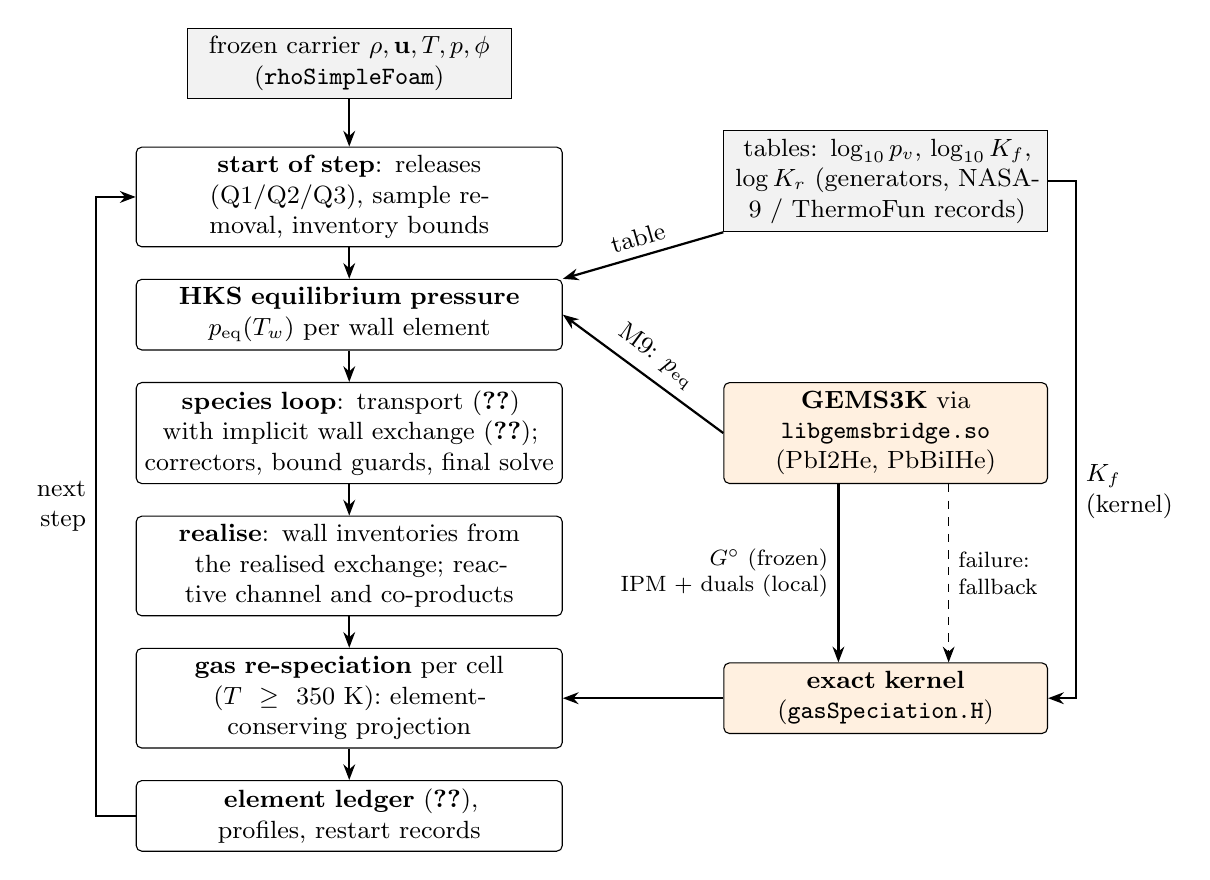
\begin{tikzpicture}[
  font=\small,
  box/.style={draw,rounded corners=2pt,align=center,minimum height=8mm,
    inner sep=3pt,text width=#1},
  box/.default=5.2cm,
  data/.style={draw,fill=gray!10,align=center,inner sep=3pt,text width=#1},
  data/.default=3.9cm,
  gems/.style={draw,fill=orange!12,rounded corners=2pt,align=center,
    inner sep=3pt,text width=#1},
  gems/.default=3.9cm,
  arr/.style={-{Stealth[length=2mm]},thick},
  fb/.style={-{Stealth[length=2mm]},dashed},
  node distance=4mm]
% solver column
\node[box] (start) {\textbf{start of step}: releases (Q1/Q2/Q3),
  sample removal, inventory bounds};
\node[box,below=of start] (peq) {\textbf{HKS equilibrium pressure}
  $p_{\rm eq}(T_w)$ per wall element};
\node[box,below=of peq] (loop) {\textbf{species loop}: transport
  \eqref{eq:transport} with implicit wall exchange \eqref{eq:halfcell};
  correctors, bound guards, final solve};
\node[box,below=of loop] (real) {\textbf{realise}: wall inventories from
  the realised exchange; reactive channel and co-products};
\node[box,below=of real] (resp) {\textbf{gas re-speciation} per cell
  ($T\ge350$ K): element-conserving projection};
\node[box,below=of resp] (ledg) {\textbf{element ledger} \eqref{eq:balance},
  profiles, restart records};
\foreach \a/\b in {start/peq,peq/loop,loop/real,real/resp,resp/ledg}
  \draw[arr] (\a) -- (\b);
\draw[arr] (ledg.west) -- ++(-0.5,0) |- node[pos=0.25,left,align=right]
  {next\\step} (start.west);
% input
\node[data,above=6mm of start] (carrier) {frozen carrier
  $\rho,\vect u,T,p,\phi$ (\texttt{rhoSimpleFoam})};
\draw[arr] (carrier) -- (start);
% thermochemistry column
\node[data] (tabs) at ($(start.east)+(4.1,0.2)$) {tables: $\log_{10}p_v$,
  $\log_{10}K_f$, $\log K_r$ (generators, NASA-9 / ThermoFun records)};
\node[gems] (bridge) at ($(loop.east)+(4.1,0)$) {\textbf{GEMS3K} via
  \texttt{libgemsbridge.so} (PbI2He, PbBiIHe)};
\node[gems] (kern) at ($(resp.east)+(4.1,0)$) {\textbf{exact kernel}
  (\texttt{gasSpeciation.H})};
\draw[arr] (tabs.south west) -- node[above,sloped]{table} (peq.north east);
\draw[arr] (bridge.west) -- node[above,sloped]{M9: $p_{\rm eq}$} (peq.east);
\draw[arr] (kern.west) -- (resp.east);
\draw[arr] (tabs.east) -- ++(0.35,0) |- node[pos=0.3,right,align=left]
  {$K_f$\\(kernel)} (kern.east);
\draw[arr] ([xshift=-6mm]bridge.south) -- node[left,align=right,font=\footnotesize]
  {$G^\circ$ (frozen)\\IPM + duals (local)} ([xshift=-6mm]kern.north);
\draw[fb] ([xshift=8mm]bridge.south) -- node[right,align=left,font=\footnotesize]
  {failure:\\fallback} ([xshift=8mm]kern.north);
\end{tikzpicture}
\caption{Data flow of one time step of \texttt{rhoFixedFlowFoam} and its
two GEMS3K coupling points. Left: operator sequence of the solver.
Right: thermodynamic inputs. The HKS equilibrium pressure comes from a
table or, optionally, from GEMS3K (M9). Gas re-speciation always ends in
the exact kernel; GEMS3K supplies either its standard states (mode
frozen) or a warm interior-point (IPM) result whose element potentials
start the kernel refinement (mode local). Dashed: fallback after a
failed or guarded GEMS3K call.}
\label{fig:dataflow}
\end{figure}

\subsection{Coupling point 1: equilibrium pressure of the HKS law}
\label{sec:peq}

For a gas--condensate pair, the solver calls GEMS3K with every condensed
species suppressed; GEMS3K then returns the homogeneous gas at the bulk
composition, and the dual activity of a suppressed condensate is its
saturation ratio $\Omega$. The equilibrium pressure is
$p_{\rm eq}=p_g10^{-\max_\varphi\log_{10}\Omega_\varphi}$ over the
pair's condensates. Two modes exist:
\begin{itemize}
\item \textbf{frozen}: cold calls at the table nodes at start-up, which
  replace the table values (PbI2He: 152 nodes in 500--1250 K, 0 failed,
  0 rejected, largest deviation from the tabulated vapour pressure
  $5.7\times10^{-5}$ decades); deterministic and restart-exact;
\item \textbf{local}: one call per wall element at the start of each
  step, at the element's temperature and its cell's composition, warm
  started from the element's own previous state. Guards fall back to the
  table below 500 K, below a mole fraction of $10^{-6}$, outside the
  GEMS3K grid, after a failed call and for results more than 0.01 decades
  from the table; a fatal error re-creates the engine. The largest
  deviation from the table in all M9 runs was $3.8\times10^{-4}$ decades;
  on the PbI$_2$ system a warm call cost about 60 $\mu$s (3.9 IPM
  iterations) with no failures in a CFD-like test loop over 1000 wall
  cells.
\end{itemize}
For Bi systems the pressure is taken from the element potentials (dual
form), which agrees with the vapour-pressure tables to
$8.37\times10^{-5}$ decades across 64 values, with additional guards
(\cref{sec:robustness}). For an ideal gas over a pure condensate of the
same formula, $p_{\rm eq}$ depends on $T$ only, so the table is exact
and GEMS3K adds no information; the Pb--Bi--I production cases therefore
use tables generated from the same thermodynamic records. GEMS3K
pressures become necessary for non-ideal or multi-component condensed
phases, which are not yet modelled.

\subsection{Coupling point 2: homogeneous gas re-speciation}

After the species loop, every cell above 350 K is projected onto the
homogeneous ideal-gas equilibrium of its element amounts: find the
partial pressures $p_i$ and element potentials $\lambda_k$ with
\begin{equation}
 \frac{p_i}{p^\circ}=K_{f,i}(T)\exp\Bigl(\sum_k\nu_{ki}\lambda_k\Bigr),
 \qquad \sum_i\nu_{ki}\frac{p_i}{RT}=b_k,
 \qquad p^\circ=10^5\units{Pa},
 \label{eq:equilibrium}
\end{equation}
and return $Y_i=M_ip_i/(\rho RT)$. Condensed phases are suppressed in
this step; condensation happens only through wall exchange. The
engine is selected in \texttt{respeciation\{engine\ldots\}}:
\begin{center}
\small
\begin{tabularx}{\textwidth}{@{}l X X@{}}
\toprule
Engine & Thermodynamic data & Solver per cell and step\\
\midrule
\texttt{kernel} & $\log_{10}K_f(T)$ table generated from the NASA-9 /
  ThermoFun records & exact element-potential Newton solver
  (\texttt{gasSpeciation.H}); no bridge needed\\
\texttt{GEMS}, \texttt{frozen} & GEMS3K standard states, cached per
  unique cell $(T,p)$ at start-up & the same exact kernel\\
\texttt{GEMS}, \texttt{local} & GEMS3K & guarded, capped warm IPM call;
  valid element potentials start the kernel refinement; canonical cold
  final refinement; kernel fallback on failure\\
\bottomrule
\end{tabularx}
\end{center}
The kernel works in logarithmic variables with a safeguarded Newton
iteration, a Schur-complement reduction of the Pb and Bi subproblems,
an extended-precision fallback for dilute bulks and bisection where
Newton steps fail to contract. Over 160,740 stored gas-map inputs it
agrees with an independent reference to $1.8\times10^{-10}$; a cold call
costs 16.2 $\mu$s on the stored 432-point set and 26--30 $\mu$s on the
broader map. The GEMS3K and open-data formation constants differ by at
most $3.69\times10^{-4}$ decades, so the engines differ in their
standard-state data at that level and otherwise solve the same
equations.

\subsection{Operator splitting and conservation}

The step is a first-order (Lie) split (\cref{fig:dataflow}): transport
with implicit wall exchange, realisation of the wall inventories, then
re-speciation once per step, never inside the corrector loop. The
re-speciated amounts are exponentials of converged potentials, absent
elements are removed exactly, cells with a non-positive element amount
are skipped and counted, and slightly negative $Y$ values are made
positive by element-conserving re-speciation rather than clipping. The
residue of every transfer between stores is booked as a CONVERSION entry
of the element ledger, so closure stays at round-off without drift.
Splitting error is first order in $\Delta t$ and is assessed by
time-step studies (\cref{sec:numstudies}).

\subsection{Robustness, guards and cost of GEMS3K}
\label{sec:robustness}

Before GEMS3K was admitted per cell, it was mapped over 321,480 calls per
run (eight Pb--Bi--I element mixes and PbI$_2$, trace fractions from
$10^{-12}$ to 0.32, 95 temperatures in 304--1244 K, one cold and three
warm calls per point, condensed species suppressed or allowed), each
compared with an exact equilibrium of GEMS3K's own $G^\circ$. Main
findings:
\begin{itemize}
\item \textbf{Failures in hot, non-dilute Bi-iodide gas.} With condensed
  species suppressed, at $T\ge500$ K, BiI$_3$ mixes fail in 0.1\%,
  6\%, 25\% and 42\% of calls at trace fractions $10^{-4}$, $10^{-3}$,
  $10^{-2}$ and $10^{-1}$; metal-rich LBE-vapour mixes in 73--100\% at
  $10^{-1}$; PbI$_2$ in at most 1\%. The interior-point criterion stalls
  at $7\times10^{-5}$--$10^{-4}$ while $G$ has converged, and the call runs
  to its 7000-iteration limit (about 45 ms). Warm starts can be worse
  than cold ones (7158 against 27 iterations).
\item \textbf{The element balance is never wrong.} None of the 311,976
  converged calls is off by more than $10^{-10}$, so the balance check
  cannot detect the silent errors, which follow the species' own mole
  fraction $x_g$: $\le4\times10^{-4}$ decades for $x_g\ge10^{-6}$, but
  0.04 at $10^{-8}$ and $\ge1$ below $10^{-11}$. The primal
  $p_{\rm eq}$ can be off by 0.33 decades at a trace fraction of
  $10^{-8}$, whereas the dual $p_{\rm eq}$ is exact to $\le10^{-9}$
  decades in every converged call.
\item \textbf{An exact solver with GEMS3K's $G^\circ$} had 0 failures in
  321,480 warm-chain and 54,720 cold calls. This motivated the
  kernel and the frozen/local designs above.
\end{itemize}
The implemented guards are: minimum temperature and mole fraction, an
upper mole-fraction bound on the trace formula units (at
$x\le3.2\times10^{-4}$ the mapped Bi-iodide gas had 0 failed calls,
against 8.5\% without the bound), the use of speciation factors only for
$x_g\ge10^{-7}$, a warm cap of 200 iterations followed by a cold retry,
and dual pressures. Fatal calls re-create the engine and invalidate the
warm states; failed calls and NaN duals take the kernel and are counted.

\begin{table}[tb]
\centering
\caption{Modelled CPU-hours of a 60 s run at 1 ms on the 228,960-cell
pipe of the cost model, for equilibrium calls (a) at the wall elements,
(b) at the walls and in cells above 700 K, (c) in every cell. For
comparison, transport costs about 40 CPU-h per paired species and
360 CPU-h for nine species.}
\label{tab:cost}
\small
\begin{tabular}{lrrr}
\toprule
Engine & (a) & (b) & (c)\\
\midrule
GEMS3K, PbI$_2$-like gas & 17 & 173 & 363\\
GEMS3K, PbI$_2$ + BiI$_3$ (with failures) & 32 & 319 & 669\\
GEMS3K, BiI$_3$-rich gas & 94 & 936 & 1960\\
Exact solver & 3.2 & 32 & 67\\
Exact solver, $G^\circ$ cached per cell & 1.4 & 13.7 & 28.6\\
\bottomrule
\end{tabular}
\end{table}

Measured on one thread (64 cells at 600--1000 K, a new $T$ every call,
$x=10^{-4}$), a warm call costs 90.8 $\mu$s with GEMS3K for PbBiIHe
(57.2 $\mu$s for PbI2He), 17.0 $\mu$s with the exact solver and 7.5
$\mu$s with the exact solver given the cell's $G^\circ$. A fit gives
about 80 $\mu$s plus 6.4 $\mu$s per IPM iteration for GEMS3K, and 1.3--3.5 ms with Bi
iodides at $x\ge10^{-3}$. On a hyperthread whose sibling runs another
job the same calls take 2.1--2.5 times as long, so production runs need
whole cores. \Cref{tab:cost} scales these costs to a full run. A tabulated surrogate of the Pb--Bi--I equilibrium was
evaluated and not recommended: a 4-D table reaches only about $10^{-2}$
decades, the minor species change by factors of 10--1000 across the
stoichiometric ridges, and the saving over the cached exact solver is
about 26 CPU-h in case (c).

\subsection{What is and what is not coupled}

\begin{itemize}
\item \textbf{Coupled:} GEMS3K equilibrium pressures for the HKS law
  (frozen or local); GEMS3K standard states or warm GEMS3K equilibria
  for the per-cell gas speciation (frozen or local); GEMS3K-generated
  systems from the same records as the solver's tables.
\item \textbf{Engine of record for the reported results:} the exact
  kernel with formation constants and vapour-pressure tables generated
  from the same standard-state records. The per-cell GEMS3K engines are a
  qualified capability (\cref{sec:gemsequiv}); in mode local the IPM
  result only starts a kernel solve and the final speciation is the
  canonical cold kernel solve, so local and frozen are bitwise identical
  (\cref{sec:pending}); this departs from the original design, in which a
  polished IPM result was to be used.
\item \textbf{Not coupled:} condensed-phase equilibrium inside GEMS3K
  (condensed phases are suppressed; condensation is wall exchange);
  source equilibrium with liquid LBE (source model Q4), which needs the
  unpublished iodine activity in LBE; feedback of species or latent heat
  on the frozen carrier; non-ideal gas or solution phases; aerosol
  nucleation; surface chemistry with steel or silica.
\end{itemize}

%======================================================================
\section{Verification}
\label{sec:verification}

\subsection{Test suite}

\texttt{tests/Alltest} runs pass/fail criteria by milestone (M0 regression
gate to M10d) and records PASS, FAIL or NOTRUN for each criterion id. The
last recorded aggregate run, \texttt{tests/Alltest all} on 2026-10-06,
gave 319 PASS, 0 FAIL and 1 NOTRUN (the v2606 compile criterion, run
separately). Later stage-specific runs gave 78 PASS, 0 FAIL, 2 NOTRUN
(M0, M9, M10c, including all nine GEMS gas-engine criteria) and 43 PASS,
0 FAIL, 13 NOTRUN (M0, M10a--d; the NOTRUNs are external-data studies not
selected and the v2606 compile). Two later kernel repairs and the
application cases were then covered by targeted checks and 19 Python
tests of the benchmark scripts. The aggregate suite was re-run on the
final sources on 2026-10-11/12 (plan section 39, item 7): 330 PASS,
0 FAIL and 3 NOTRUN, after six parallel pipe criteria that had stopped
at the 30-minute MPI time limit on a heavily loaded machine passed with
a longer limit. The NOTRUNs are the v2606 regression gate (passed in a
separate v2606 run, 27 PASS), a bridge-provenance criterion that is
NOTRUN by design, and a timing benchmark refused on the loaded machine.
Criteria needing licensed Bi--I data are NOTRUN without the external
files.

Selected criteria: the half-cell wall law converges at order 2.0 on a
Graetz problem with a Robin wall (P\'eclet 5, Biot 1 and 50), with
errors of the developed decay rate of $8\times10^{-7}$ to
$2\times10^{-4}$; two independent pairs equal two single-pair runs byte
for byte, serial and on four ranks; binary restarts are byte-identical;
1\% deposition onsets of a 1000--350 K channel agree with an independent
plug-flow equilibrium within 5.9 K (gate 10 K), and the five onsets of
the reactive metal-vapour channel within 3.9 K for both BiI(g) data
sets.

\subsection{Conservation}

\begin{center}
\small
\begin{tabular}{lll}
\toprule
Quantity (relative to supplied material) & Production (19 runs) &
  Follow-up (60 runs)\\
\midrule
Largest raw element residue $R_k$ & $\ProductionResidue$ &
  $8.85\times10^{-13}$\\
Largest accounted closure & $1.12\times10^{-15}$ & $9.60\times10^{-16}$\\
Largest linear-solver defect & $1.45\times10^{-12}$ & $8.64\times10^{-13}$\\
\bottomrule
\end{tabular}
\end{center}
The baseline logs report no gas-equilibrium failures and a maximum
equilibrium element residue of $6.43\times10^{-16}$. These figures
establish conservation of the discrete model, not physical accuracy.

\subsection{Numerical studies}
\label{sec:numstudies}

\Cref{tab:numerical} lists the iodine-profile changes $E_{L1}$ (percent
of the reference deposit, 1 cm bins) between successive meshes and
schemes, and for halving the time step. Halving the 2 ms step changes
profiles by \TimeMin--0.3228\%, and eight instead of three species
correctors over a full 60 s run by at most \IterSteelHigh\%. The spatial
error is larger and is dominated by first-order upwind diffusion: at
equal mesh upwind differs from the bounded \texttt{limitedLinear} scheme
by \UpLLFour--\UpLLOne\% in the most sensitive case, whereas two bounded
schemes differ by at most \VLSteelMax\%. On a fourth level (93,312
cells) that case changes by \SteelLLThree\%, its total deposit by
\SteelTotalThree\% and its centroid by less than 1 mm. Apparent orders
(\SteelOrderOne{} and \SteelOrderTwo) are inconsistent, so no formal grid
convergence index is claimed. Production runs therefore use
\texttt{Gauss limitedLinear 1} on 41,472 cells.

\begin{table}[tb]
\centering
\caption{Iodine profile changes $E_{L1}$ (\%) between successive mesh
levels at 2 ms, relative to the finer level, and for halving the time
step (18,432 cells, upwind). Steel cases are Q2 (Liu et al.\ steel
column); the shifted-BiI case uses 1\% metal saturation. A dash marks a
combination not run. (Generated table of the methods manuscript.)}
\label{tab:numerical}
\small\begin{tabular}{llrrrr}
\toprule
Case & Scheme & 8,192$\to$18,432 & 18,432$\to$41,472 & 41,472$\to$93,312 & 2$\to$1 ms \\
\midrule
Pure PbI$_2$ & upwind & 6.57 & 5.06 & 3.68 & 0.0043 \\
 & limitedLinear & 5.70 & 2.15 & -- & -- \\
 & van Leer & 4.94 & 2.23 & -- & -- \\
\midrule
Steel, shifted BiI & upwind & 10.47 & 10.58 & 2.13 & 0.1536 \\
 & limitedLinear & 15.35 & 8.95 & 1.98 & -- \\
 & van Leer & 16.83 & 9.17 & -- & -- \\
\midrule
Steel Q2, 0.1\% & upwind & 9.02 & 5.26 & 7.30 & 0.2326 \\
\midrule
Steel Q2, 1\% & upwind & 9.72 & 2.06 & 6.68 & 0.3228 \\
\bottomrule
\end{tabular}

\end{table}

\subsection{Equivalence of the gas engines (qualification channel)}
\label{sec:gemsequiv}

Case \slug{pbbi-gems-speciation} is a synthetic 1173--350 K channel with
a prescribed PbI$_2$/BiI$_3$ source (iodine mole fraction
$3.9\times10^{-6}$), 1 ms steps for 3 s, run with all three engines
(\texttt{verification.json}, \texttt{qualification.json}):
\begin{center}
\small
\begin{tabular}{lr}
\toprule
Quantity & Value\\
\midrule
Deposit L1, frozen vs kernel, PbI$_2$ / BiI$_3$ (1 cm bins) &
  $1.03\times10^{-10}$ / $1.06\times10^{-7}$ (gate $10^{-3}$)\\
Deposit L1, local vs frozen & 0 (gate $10^{-9}$)\\
Maximum element closure & $6.66\times10^{-16}$\\
Local GEMS3K calls; mean cost incl.\ both refinements & 5,814,420;
  132.24 $\mu$s (gate 150 $\mu$s)\\
Reduced map (936 points): species error of refined result &
  $6.82\times10^{-10}$\\
Reduced map: element error; raw IPM failures & $5.03\times10^{-16}$; 0\\
Reduced map: points refused by the guards & 236\\
Reduced map: largest raw IPM deviation (bulk $x=10^{-10}$) & 0.64 decades\\
GEMS3K vs open-data $\log_{10}K_f$ & $\le3.69\times10^{-4}$ decades\\
Serial / four-rank closure; frozen restarts & $\le10^{-14}$; byte-identical\\
\bottomrule
\end{tabular}
\end{center}
The raw IPM deviations of up to 0.64 decades at trace dilution are the
reason why mode local passes every IPM result through the exact kernel,
which computes the final speciation (\cref{sec:pending}). Injected fatal and NaN-dual failures are counted, re-create the
engine where required, and leave the fields byte-identical to the frozen
kernel fallback. These are numerical results under provisional inputs
(synthetic carrier ramp and common diffusivity).

\subsection{Production-scale per-cell GEMS3K run}
\label{sec:pending}

The full production case of the Liu et al.\ steel experiment (Q2
source, 1\% metal saturation; $576\times72=41{,}472$ cells,
\texttt{Gauss limitedLinear 1}, 60\,s at 2\,ms) was repeated with the
GEMS3K engines, changing only the \texttt{respeciation} engine
(\cref{tab:pending}). The bridge-enabled solver was built from the same
solver sources as the production binary; run serially with the kernel
engine it reproduces the production ledgers bit for bit. The GEMS3K runs
used 8 MPI ranks (axial slabs, CPU-bound); an 8-rank kernel run with the
same decomposition separates parallel round-off from the engine effect.

\begin{table}[tb]
\centering
\caption{Production-scale comparison of the gas engines (records in
\texttt{run/024-liu2025/gems\_engine\_check/}).}
\label{tab:pending}
\small
\begin{tabular}{lllll}
\toprule
Quantity & kernel, serial & kernel, 8 ranks & GEMS frozen & GEMS local\\
\midrule
Wall-clock time [h] & 25.04 & 6.37 & 6.74 & 10.73\\
CPU time [core-h] & 25.0 & 50.9 & 53.9 & 85.8\\
GEMS3K interior-point calls & -- & -- & -- & $5.145\times10^{8}$\\
Call failures / engine re-creations & -- & -- & -- & 0 / 0\\
Lower-guard activations (trace $<10^{-12}$) & -- & -- & -- & 14.0\%\\
Mean cost per call [$\mu$s] & -- & -- & -- & 150.8\\
Largest element closure & $5.4\times10^{-16}$ & $5.5\times10^{-16}$ & $5.8\times10^{-16}$ & $5.8\times10^{-16}$\\
Iodine profile $E_{L1}$ vs serial kernel & 0 & $1.8\times10^{-4}$ & $9.9\times10^{-5}$ & $9.9\times10^{-5}$\\
BiI$_3$ share of iodide iodine [\%] & 94.5837 & -- & 94.5841 & 94.5841\\
\bottomrule
\end{tabular}
\end{table}

Using GEMS3K's standard-state energies in every re-speciated cell
(19,944 distinct cell states; formation constants within
$3.64\times10^{-4}$ decades of the kernel table) changes the iodine,
PbI$_2$, BiI$_3$, Pb and Bi deposit profiles by at most
$2.1\times10^{-4}$ (relative $L_1$ of the 1\,cm profiles), the BiI$_3$
share of iodide iodine by 0.0004 percentage points and the peak
temperatures by less than 0.003\,K. Parallel round-off alone is of the
same order (up to $2.7\times10^{-4}$); at equal decomposition the engine
effect is at most $1.8\times10^{-4}$.

Modes frozen and local give bitwise identical results in all fields,
profiles and ledger records. This follows from the implementation: in
mode local the warm GEMS3K interior-point result starts a kernel solve,
and the final speciation is then computed by the canonical cold kernel
solve from the same GEMS3K thermodynamic data. The 514.5 million
GEMS3K calls (none failed) therefore demonstrate the robustness and cost
of per-cell GEMS3K calls at production scale (59\% above the frozen
engine), but they do not shape the result. The coupling as used at
production scale is GEMS3K thermodynamics per cell with an exact,
element-conserving equilibrium solve; a GEMS3K-solved equilibrium, and
condensed phases inside GEMS3K, are not demonstrated.

%======================================================================
\section{Modelling applications}
\label{sec:applications}

\subsection{Liu et al.\ (2025): Pb--Bi--I deposition from LBE}

Liu et al.\ \cite{Liu2025chemical} evaporated PbI$_2$ and iodine-containing
LBE into helium in steel (4.8 mm) and silica (5.0 mm) columns. The
model transports the nine Pb--Bi--I gases, with HKS exchange of
PbI$_2$ and BiI$_3$ ($C_e=s_i=\alpha_i=1$, half-cell resistance), the Pb
and Bi metal channels and the reactive BiI channel, in a frozen carrier
built from the digitised wall temperatures. 15 baseline and 64 follow-up
cases (60 s; four flow-stop cases continued to 80 s) and 19 production
re-runs were completed. Source Q1
releases PbI$_2$ and BiI$_3$ at the mean rate of the deposited masses,
so the split is imposed; Q2 releases elements plus LBE metal vapour at
an unmeasured fraction $\beta$ of saturation, so the split emerges.

\begin{figure}[tb]
\centering
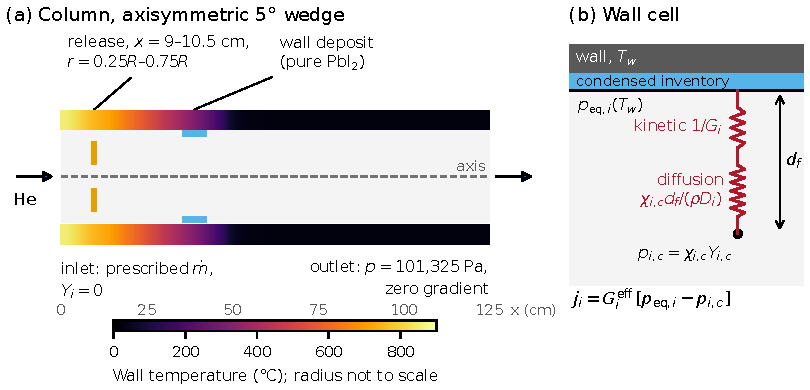
\includegraphics[width=\textwidth]{experiment_schematic.pdf}
\caption{Computational geometry of the Liu et al.\ columns: a 1.25 m
tube, represented by an axisymmetric 5$^\circ$ wedge, with a prescribed
source region near the hot end. The boat itself is not resolved.}
\label{fig:geometry}
\end{figure}

\begin{table}[tb]
\centering
\caption{Q1 iodide maxima on the production mesh compared with the
published peaks \cite{Liu2025chemical}. Subscript bin: 1 cm binned
maximum; 3: maximum of the 3 cm smoothed profile; $T_{\rm c}$: wall
temperature at the deposit centroid. Positions in cm, temperatures in
$^\circ$C; experimental ranges are those printed in the paper.}
\label{tab:peaks}
\small\begin{tabular}{llrrrrrrr}
\toprule
Case & Species & $x_{\rm exp}$ & $x_{\rm bin}$ & $x_{3}$ & $T_{\rm exp}$ & $T_{\rm bin}$ & $T_{3}$ & $T_{\rm c}$ \\
\midrule
Pure PbI$_2$, steel & \ce{PbI2} & 36 & 36 & 37 & 368$\pm$18 & 366.5 & 350.5 & 348.7 \\
LBE, steel & \ce{PbI2} & 51 & 51 & 52 & 288$\pm$18 & 288.1 & 269.2 & 274.5 \\
LBE, steel & \ce{BiI3} & 57 & 57 & 58 & 154$\pm$14 & 166.9 & 138.8 & 158.1 \\
LBE, silica & \ce{PbI2} & 51 & 56 & 56 & 306$\pm$24 & 287.8 & 287.8 & 288.8 \\
LBE, silica & \ce{BiI3} & 59 & 63 & 64 & 127$\pm$39 & 152.8 & 119.8 & 147.1 \\
\bottomrule
\end{tabular}

\end{table}

Key results (\cref{tab:peaks,fig:thermo}):
\begin{itemize}
\item All five binned Q1 peak temperatures lie inside the printed
  ranges. The smoothed and centroid temperatures lie at or near the
  lower limits, and the silica maxima lie 5 and 4 cm downstream of the
  measured positions. The Q1 BiI$_3$ share of deposited iodide iodine
  (65.34\% steel, 28.68\% silica, against 65.63\% and 29.03\% measured) is
  conditioned on source masses taken from the same deposits and is not a
  prediction.
\item The silica temperature curve and its printed peak labels disagree
  by about 63 K and 108 K. Two input-derived shifts of the curve
  ($-4.10$ and $-4.65$ cm) raise the profile overlap from 6.13\% to
  77.80\% and 73.26\%; they are hypotheses, not corrections, and their
  ranking reverses between advection schemes.
\item \textbf{Main sensitivity: BiI(g) thermodynamics.} At 1\% metal
  saturation in steel, the baseline (Barin) data give a BiI$_3$ share of
  94.58\%; raising the BiI(g) Gibbs energy by $29\units{kJ\,mol^{-1}}$
  gives 2.01\%. With this shift the open-data gas speciation comes close
  to Liu's published equilibrium figures (best shifts 29--30
  kJ\,mol$^{-1}$; rms deviation 0.014--0.047 instead of 0.270--0.368). The shift is a sensitivity surrogate, not a qualified
  record. The split also depends on the unmeasured metal loading, so no
  branch is selected.
\item Input sensitivities (iodine profile, 18,432-cell upwind
  differences): gas diffusivity up to 14.20\%, flow reference
  conditions 5.09--10.93\%, iodide accommodation up to 4.21\%, source
  position at most 0.19\%. Diffusion, not interfacial kinetics, limits
  wall exchange (wall Damk\"ohler number $1.4\times10^3$--$2.9\times10^3$
  at $\alpha=1$).
\end{itemize}

\begin{figure}[tb]
\centering
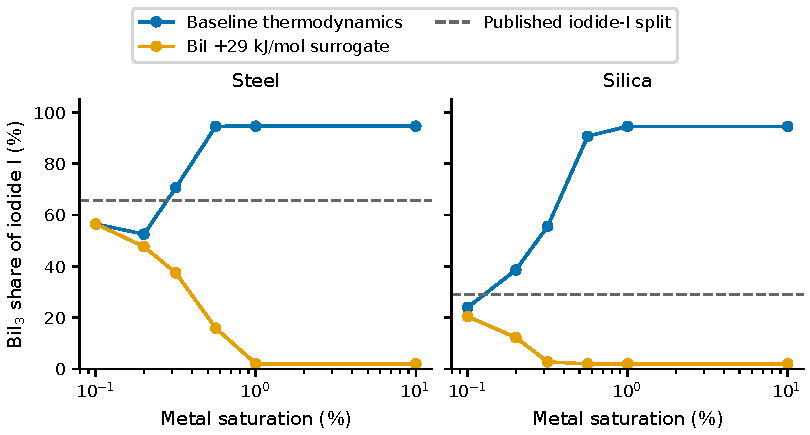
\includegraphics[width=\textwidth]{source_thermodynamics.pdf}
\caption{Conditional sensitivity of the BiI$_3$ share of deposited iodide
iodine to metal loading $\beta$ and BiI(g) thermodynamics, for the steel
and silica LBE cases (source Q2). Dashed grey lines: published BiI$_3$
share after excluding KI \cite{Liu2025chemical}. The $+29$ kJ/mol branch
is a surrogate perturbation.}
\label{fig:thermo}
\end{figure}

\subsection{Lobresco et al.\ (2026): PbI$_2$ head-to-head}

The five PbI$_2$ experiments of Lobresco et al.\
\cite{Lobresco2026assessment} (helium flows 5, 106 and 540 mL/min,
durations 6--300 s) were run without adjusting any parameter: HKS with
$C_e=\alpha=1$ and the half-cell resistance, the digitised published
wall temperatures, an evaporating sample, \LobCellsProd{} cells and
limited-linear advection. With the paper's 1\%-of-peak onset rule
(\cref{tab:lobresco,fig:lobresco}) the onset temperatures differ from the
measurements by \LobDiffA, \LobDiffB, \LobDiffC, \LobDiffD{} and
\LobDiffE{} K, an RMS of \LobRMS{} K against \LobRMSTemp{} K for both
published models; the two meshes agree within \LobCoarse{} K. The
computed peaks lie \LobShiftMin--\LobShiftMax{} cm upstream of the
measured ones. Not represented: the flow stop and withdrawal at the end
of the experiment, the boat, and the non-dilute source region (PbI$_2$
mole fraction 0.33--0.36 next to the sample). This is an independent
comparison with published measurements and models, not a validation.

\begin{table}[tb]
\centering
\caption{Deposition-onset temperatures for the five PbI$_2$ experiments
of Lobresco et al.\ \cite{Lobresco2026assessment}: flow (mL/min,
standard), duration (s), measured onset (K), and onset minus measurement
(K) for this work and for the temperature-based and vapour-pressure-based
models of that paper. $\Delta x_{\rm pk}$: computed minus measured peak
(cm); $L_1/n_0$: absolute profile difference over the sample amount.}
\label{tab:lobresco}
\small\begin{tabular}{lrrrrrrrr}
\toprule
Case & $\dot V$ & $t$ & $T_{\rm exp}$ & This work & Temp.-based & Vap.-press. & $\Delta x_{\rm pk}$ & $L_1/n_0$ \\
\midrule
T106\_6 & 106 & 6 & 814 & +26 & $-$39 & +27 & $-$4 & 0.89 \\
T106\_60 & 106 & 60 & 723 & +19 & $-$10 & +37 & $-$2 & 0.66 \\
T106\_300 & 106 & 300 & 667 & +16 & $-$1 & +34 & $-$2 & 0.88 \\
T5\_60 & 5 & 60 & 847 & $-$11 & $-$60 & $-$50 & $-$1 & 0.37 \\
T540\_60 & 540 & 60 & 700 & $-$14 & $-$30 & $-$15 & $-$1 & 0.47 \\
\midrule
RMS &  &  &  & 18 & 35 & 35 &  &  \\
\bottomrule
\end{tabular}

\end{table}

\begin{figure}[tbp]
\centering
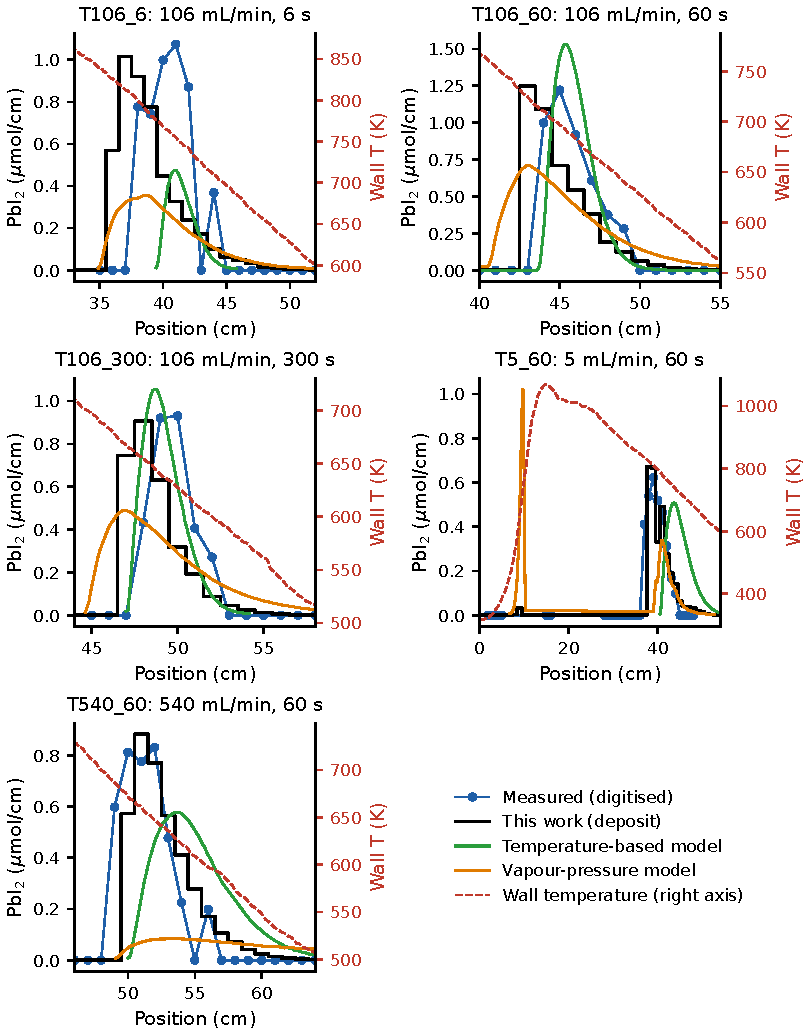
\includegraphics[width=0.7\textwidth]{lobresco_comparison.pdf}
\caption{Deposited PbI$_2$ for the five experiments of Lobresco et al.:
measured profiles and the two published model results (digitised,
adapted under CC BY 4.0 \cite{Lobresco2026assessment}), and this work at
the end of each experiment. Dashed red: digitised wall temperature.}
\label{fig:lobresco}
\end{figure}

%======================================================================
\section{Code availability and use}
\label{sec:availability}

{\sloppy\paragraph{Repository.} Solver, bridge, generators, benchmarks, cases and
tests are in the LESTO repository, \url{https://github.com/JanKren/LESTO}
\TC{repository access, release tag or commit to be cited, and the
licence of the repository's own code}:
\path{applications/rhoFixedFlowFoam} (solver, \path{tests/},
design and decision record \path{doc/phase-change-plan.md}),
\path{thermochemistry/} (\path{gemsbridge}, \path{systems},
\path{benchmarks/liu2025}, \path{benchmarks/lobresco2026}), and
\path{run/}.\par}

\paragraph{Case ladder.} The cases in \texttt{run/} add one capability
at a time. Because they are being renumbered into a continuous ladder,
they are cited here by slug:
\begin{center}
\small
\begin{tabularx}{\textwidth}{@{}>{\raggedright\arraybackslash}p{0.5\textwidth} X@{}}
\toprule
Slug & Capability\\
\midrule
\slug{first-pipe-flow-simpleFoam} \ldots{}
\slug{variable-properties-high-temperature} & carrier development:
  laminar pipe, parabolic inlet, energy, variable wall temperature,
  density and properties\\
\slug{one-species-transport-rhoFixedFlowFoam}, \slug{variable-diffusivity},
\slug{handles-solid-species}, \slug{coupled-species-sources} & frozen-carrier
  transport, PbI$_2$--He diffusivity, condensed species, coupled sources\\
\slug{temperature-model}, \slug{paper-temperature-model} & temperature-based
  deposition law; paper-mode carrier\\
\slug{hks-inventory}, \slug{hks-gems-local} & HKS law with an evaporating
  inventory; $p_{\rm eq}$ from GEMS3K (mode local, M9)\\
\slug{pbi2-bii3-channel}, \slug{pbbi-gas-speciation},
\slug{pbbi-gems-speciation}, \slug{lbe-metal-vapour} & two iodide pairs;
  kernel re-speciation; GEMS3K gas engines; metal vapour and reactive
  channels\\
\slug{liu2025}, \slug{lobresco2026} & the applications of
  \cref{sec:applications}\\
\bottomrule
\end{tabularx}
\end{center}

\paragraph{Building and running.} With OpenFOAM v2412 sourced:
\begin{itemize}
\item default solver: \texttt{applications/rhoFixedFlowFoam/Allwmake};
\item with GEMS3K: build the static GEMS3K and the bridge
  (\texttt{build-gems3k-static.sh}, \texttt{make \&\& make check}, conda-forge
  toolchain), then\\ \path{export LESTO_GEMSBRIDGE=<LESTO>/thermochemistry/gemsbridge}\\
  and \texttt{Allwmake}; \texttt{rhoFixedFlowFoam -help} states whether the
  bridge is compiled in. The bridge is machine-specific (glibc $\ge2.34$)
  and is rebuilt on each machine, e.g.\ on the PSI cluster Merlin7;
\item cases: \texttt{./Allrun} in the case directory, with the external
  thermodynamic paths in environment variables
  (\texttt{LESTO\_M10\_SYSTEM}, \texttt{LESTO\_M10\_DATA},
  \texttt{LESTO\_M10E\_NASA}, \texttt{LESTO\_M10E\_THERMOFUN}) and, for the
  Liu cases, explicit flow-reference conditions;
\item tests: \texttt{tests/Alltest <milestones>} or \texttt{all}.
\end{itemize}

\paragraph{Data licences.} GEMS3K is LGPL-3.0; the NASA CEA records and
the files derived from them are Apache-2.0. The Bi--I data derive from
HERACLES (ThermoHub, GPL-3.0; Barin \cite{Barin1995thermochemical}); their
provenance and redistribution terms are unconfirmed, so no Bi--I record
or derived table is in the repository and the Bi--I criteria and cases
need the external files. JANAF-derived files are internal checks only and
data derived from HSC Chemistry are not redistributable. The digitised
curves of Liu et al.\ and Lobresco et al.\ are adapted under the source
papers' CC BY 4.0 licences.

%======================================================================
\section{Limitations and outlook}
\label{sec:outlook}

\paragraph{Limitations.}
\begin{itemize}
\item \textbf{Engine of record.} The reported results use the exact
  kernel; per-cell GEMS3K is qualified on a channel but not yet shown at
  production scale (\cref{sec:pending}).
\item \textbf{Physics not represented.} Frozen carrier (no buoyancy,
  latent heat or species feedback), ideal gas, no condensed-phase
  equilibrium in cells, no LBE source equilibrium, prescribed release,
  no aerosol formation, Soret diffusion, surface chemistry, KI, water or
  oxygen chemistry; the BiI wall channel is irreversible and
  phenomenological; instantaneous gas equilibrium replaces unmeasured
  kinetics.
\item \textbf{Inputs.} The +29 kJ/mol BiI(g) value is a surrogate; the
  BiI$_3$ liquid record is constructed; the Bi data provenance is
  unqualified. Missing experimental inputs: original temperature
  profiles and scan coordinates, flow-controller reference conditions,
  release histories, boat geometry, surface coefficients.
\item \textbf{Numerics.} The indicative spatial error of the profile on
  the production mesh is 2.5--3.6\% for the most sensitive case; no
  formal mesh independence is claimed. The source region of the Lobresco
  cases is not dilute.
\end{itemize}

\paragraph{Outlook.}
\begin{itemize}
\item Complete the production-scale GEMS3K run and the aggregate test
  re-run on the final sources.
\item Obtain the missing experimental inputs and a qualified BiI(g)
  record before any predicted iodide split is used; clarify the Bi data
  licence.
\item Extend GEMS3K coupling to phases where it adds information beyond
  the tables: non-ideal or multi-component condensates, and source
  equilibrium with liquid LBE once iodine activity data are available.
\item Machine-learning and reduced-order surrogates of the coupled
  model are planned in a later phase of Task 3.4. The cost analysis
  above indicates that for the Pb--Bi--I gas alone a tabulated surrogate
  gains little over the cached exact solver, so surrogates are expected
  to matter for larger systems and for reactor-scale transport.
\end{itemize}

%======================================================================
\small\setlength{\bibsep}{2pt}
\bibliographystyle{unsrtnat}
\bibliography{../../manuscript/references}

\end{document}
